\newpage
\section{Auswertung}

Um die aufgenommenen Daten zu analysieren werden die Python~\cite{python} Pakete NumPy~\cite{numpy} und SciPy~\cite{scipy} verwendet,
wobei Matplotlib~\cite{matplotlib} zum Erstellen von Grafiken und zudem Uncertainties~\cite{uncertainties} zur automatisierten
Fehlerfortpflanzung in linearer Ordnung dienen.



\subsection{Verzögerungszeit}

\begin{figure}[H]
	\centering
	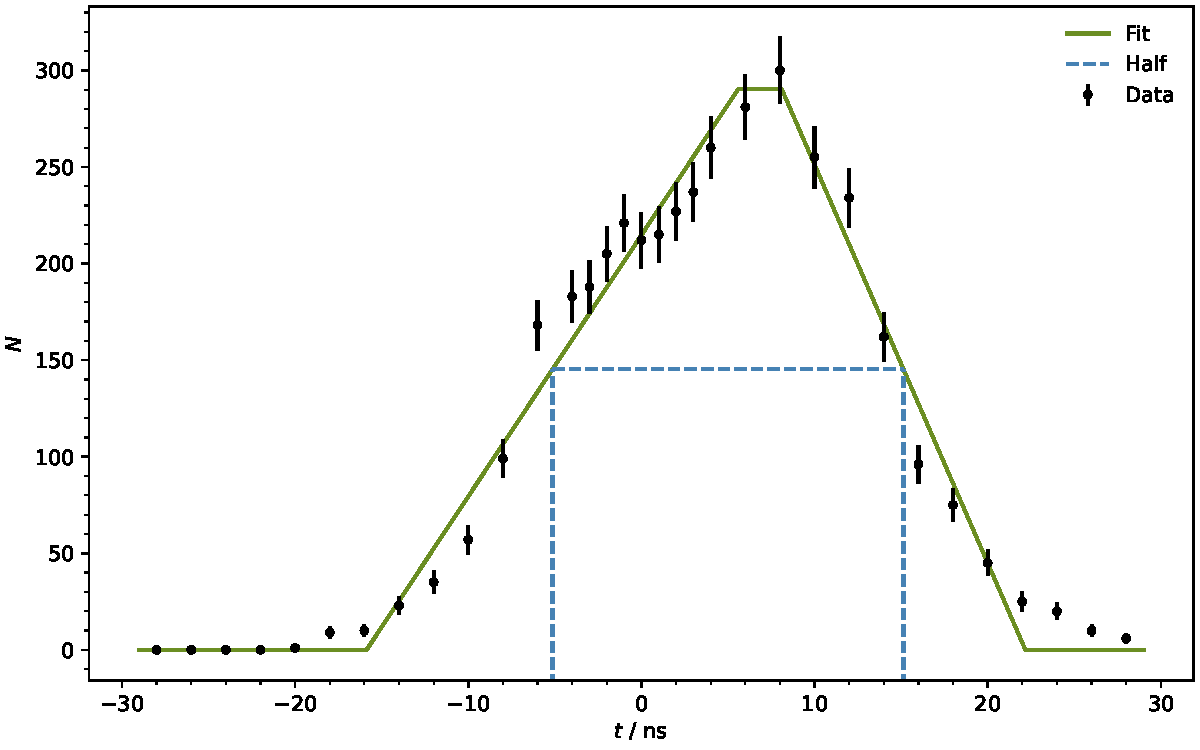
\includegraphics[width=\textwidth]{build/delay.pdf}
	\caption{.}
	\label{fig:delay}
\end{figure}

\begin{equation*}
	a = \qty{1.7+-0.1}{\per\nano\second}
\end{equation*}

\begin{align*}
	b &= \qty{-11.6+-0.3}{\nano\second} \: , & c &= \qty{-0.1+-0.4}{\nano\second} \: , \\
	d &= \qty{8.1+-0.9}{\nano\second} \: , & e &= \qty{17.3+-0.3}{\nano\second}
\end{align*}

\begin{equation*}
	N_\text{Plateau} = \num{20+-1}
\end{equation*}

\begin{equation*}
	T_\text{Plateau} = \qty{5.3+-0.5}{\nano\second}
\end{equation*}

\begin{align*}
	t_\text{links} = \qty{-5.9+-0.2}{\nano\second} \: , && t_\text{rechts} = \qty{11.2+-0.2}{\nano\second}
\end{align*}

\begin{equation*}
	T_\text{Hälfte} = \qty{20.3+-0.8}{\nano\second}
\end{equation*}

\begin{equation*}
	T_\text{Auflösung} = \qty{11.8+-0.3}{\nano\second}
\end{equation*}



\subsection{Kanalkalibration}

\begin{figure}[H]
	\centering
	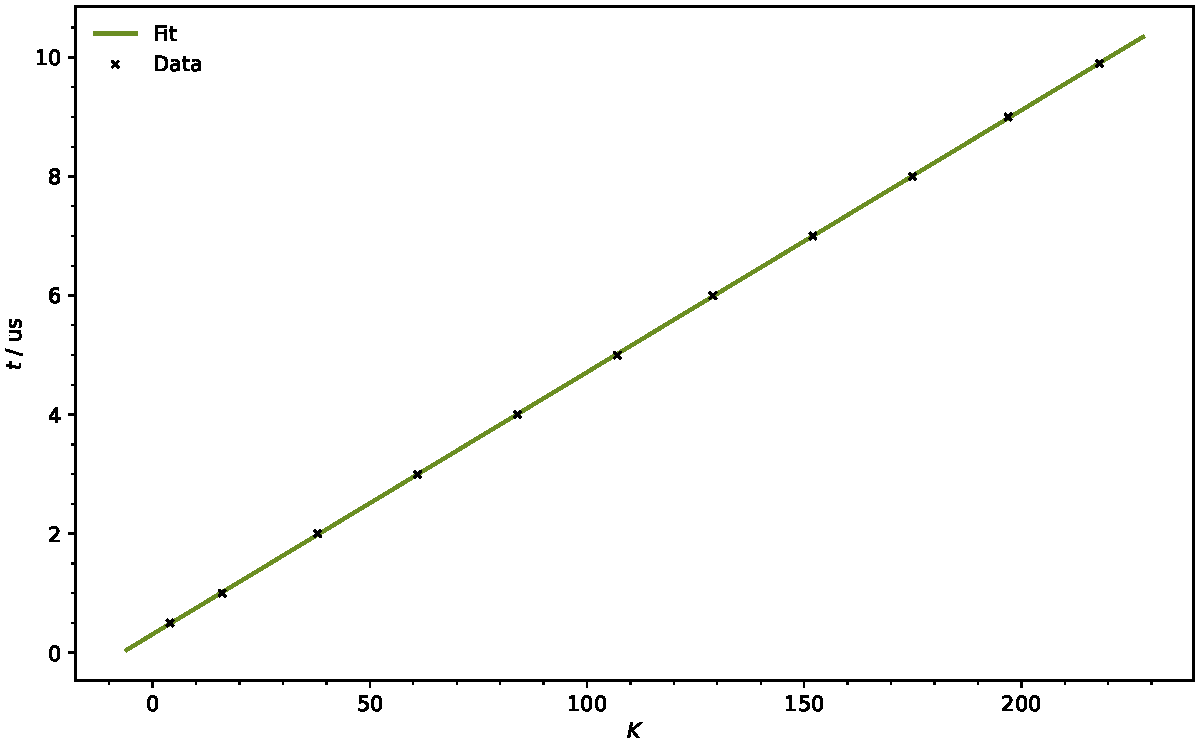
\includegraphics[width=\textwidth]{build/calibration.pdf}
	\caption{.}
	\label{fig:calibration}
\end{figure}

\begin{equation*}
	t(K) = AK + B
\end{equation*}

\begin{align*}
	A = \qty{0.02167+-0.00001}{\micro\second} \: , && B = \qty{0.313+-0.008}{\micro\second}
\end{align*}



\subsection{Langzeitmessung}

\begin{figure}[H]
	\centering
	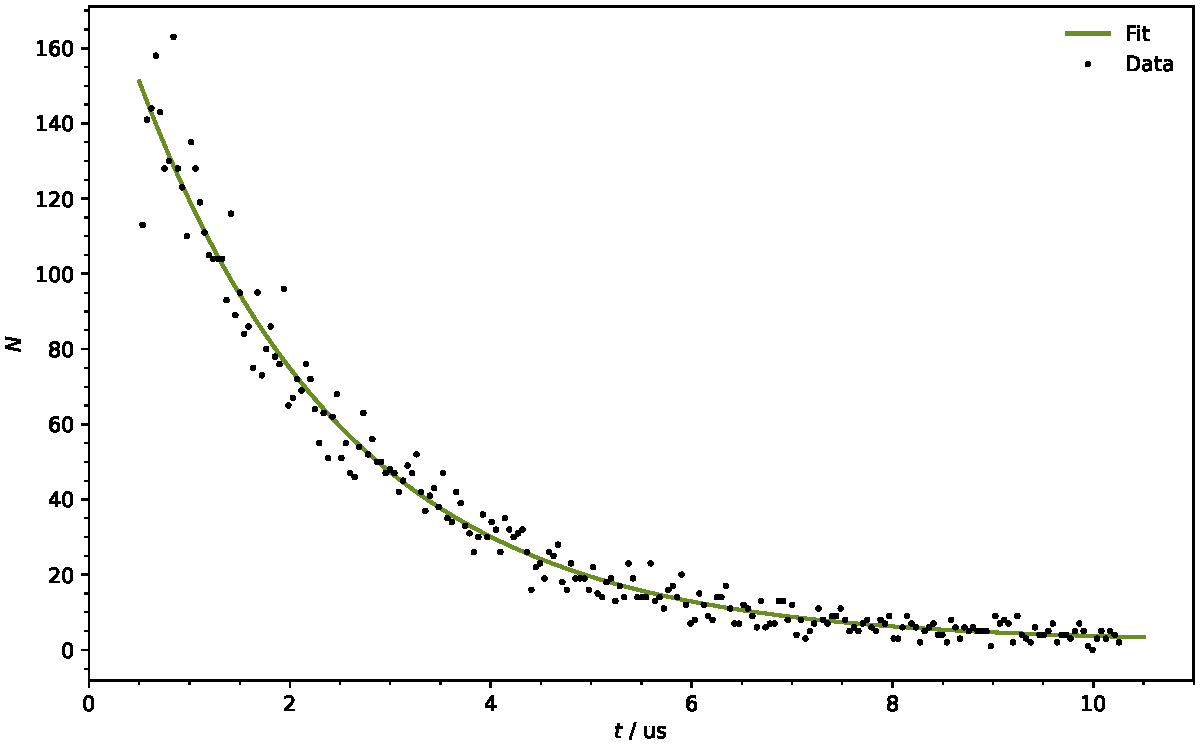
\includegraphics[width=\textwidth]{build/lifetime.pdf}
	\caption{.}
	\label{fig:lifetime}
\end{figure}

\begin{equation*}
	N(t) = m + ne^{-\lambda t}
\end{equation*}

\begin{align*}
	m = \num{2.03(0.01)} \: , && n = \num{186.1+-2.7}
\end{align*}

\begin{equation*}
	\lambda = \qty{0.44+-0.02}{\per\micro\second}
\end{equation*}

\begin{equation*}
	\tau = \qty{1.03+-0.03}{\micro\second}
\end{equation*}



\subsection{Hintergrundrate}

\begin{align*}
	T_\text{such} &= \qty{10}{\micro\second} \: , & T_\text{mess} &= \qty{158234}{\second} \: , \\
	N_\text{start} &= \num{4509112} \: , & N_\text{stopp} &= \num{17526}
\end{align*}

\begin{equation*}
	\langle N \rangle = N_\text{stopp} \frac{T_\text{such}}{T_\text{mess}}
\end{equation*}

\begin{equation*}
	P_k = \pfrac{\langle N \rangle ^k}{k!} e^{-\langle N \rangle}
\end{equation*}

\begin{equation*}
	P_1 = \qty{0.0191}{\percent}
\end{equation*}

\begin{equation*}
	O = \num{562}
\end{equation*}

\num{512}

\begin{equation*}
	M = \num{2.5}
\end{equation*}
